\documentclass[]{elsarticle} %review=doublespace preprint=single 5p=2 column
%%% Begin My package additions %%%%%%%%%%%%%%%%%%%
\usepackage[hyphens]{url}

  \journal{Forest Ecology and Management} % Sets Journal name


\usepackage{lineno} % add
\providecommand{\tightlist}{%
  \setlength{\itemsep}{0pt}\setlength{\parskip}{0pt}}

\usepackage{graphicx}
\usepackage{booktabs} % book-quality tables
%%%%%%%%%%%%%%%% end my additions to header

\usepackage[T1]{fontenc}
\usepackage{lmodern}
\usepackage{amssymb,amsmath}
\usepackage{ifxetex,ifluatex}
\usepackage{fixltx2e} % provides \textsubscript
% use upquote if available, for straight quotes in verbatim environments
\IfFileExists{upquote.sty}{\usepackage{upquote}}{}
\ifnum 0\ifxetex 1\fi\ifluatex 1\fi=0 % if pdftex
  \usepackage[utf8]{inputenc}
\else % if luatex or xelatex
  \usepackage{fontspec}
  \ifxetex
    \usepackage{xltxtra,xunicode}
  \fi
  \defaultfontfeatures{Mapping=tex-text,Scale=MatchLowercase}
  \newcommand{\euro}{€}
\fi
% use microtype if available
\IfFileExists{microtype.sty}{\usepackage{microtype}}{}
\bibliographystyle{elsarticle-harv}
\usepackage{color}
\usepackage{fancyvrb}
\newcommand{\VerbBar}{|}
\newcommand{\VERB}{\Verb[commandchars=\\\{\}]}
\DefineVerbatimEnvironment{Highlighting}{Verbatim}{commandchars=\\\{\}}
% Add ',fontsize=\small' for more characters per line
\usepackage{framed}
\definecolor{shadecolor}{RGB}{248,248,248}
\newenvironment{Shaded}{\begin{snugshade}}{\end{snugshade}}
\newcommand{\KeywordTok}[1]{\textcolor[rgb]{0.13,0.29,0.53}{\textbf{#1}}}
\newcommand{\DataTypeTok}[1]{\textcolor[rgb]{0.13,0.29,0.53}{#1}}
\newcommand{\DecValTok}[1]{\textcolor[rgb]{0.00,0.00,0.81}{#1}}
\newcommand{\BaseNTok}[1]{\textcolor[rgb]{0.00,0.00,0.81}{#1}}
\newcommand{\FloatTok}[1]{\textcolor[rgb]{0.00,0.00,0.81}{#1}}
\newcommand{\ConstantTok}[1]{\textcolor[rgb]{0.00,0.00,0.00}{#1}}
\newcommand{\CharTok}[1]{\textcolor[rgb]{0.31,0.60,0.02}{#1}}
\newcommand{\SpecialCharTok}[1]{\textcolor[rgb]{0.00,0.00,0.00}{#1}}
\newcommand{\StringTok}[1]{\textcolor[rgb]{0.31,0.60,0.02}{#1}}
\newcommand{\VerbatimStringTok}[1]{\textcolor[rgb]{0.31,0.60,0.02}{#1}}
\newcommand{\SpecialStringTok}[1]{\textcolor[rgb]{0.31,0.60,0.02}{#1}}
\newcommand{\ImportTok}[1]{#1}
\newcommand{\CommentTok}[1]{\textcolor[rgb]{0.56,0.35,0.01}{\textit{#1}}}
\newcommand{\DocumentationTok}[1]{\textcolor[rgb]{0.56,0.35,0.01}{\textbf{\textit{#1}}}}
\newcommand{\AnnotationTok}[1]{\textcolor[rgb]{0.56,0.35,0.01}{\textbf{\textit{#1}}}}
\newcommand{\CommentVarTok}[1]{\textcolor[rgb]{0.56,0.35,0.01}{\textbf{\textit{#1}}}}
\newcommand{\OtherTok}[1]{\textcolor[rgb]{0.56,0.35,0.01}{#1}}
\newcommand{\FunctionTok}[1]{\textcolor[rgb]{0.00,0.00,0.00}{#1}}
\newcommand{\VariableTok}[1]{\textcolor[rgb]{0.00,0.00,0.00}{#1}}
\newcommand{\ControlFlowTok}[1]{\textcolor[rgb]{0.13,0.29,0.53}{\textbf{#1}}}
\newcommand{\OperatorTok}[1]{\textcolor[rgb]{0.81,0.36,0.00}{\textbf{#1}}}
\newcommand{\BuiltInTok}[1]{#1}
\newcommand{\ExtensionTok}[1]{#1}
\newcommand{\PreprocessorTok}[1]{\textcolor[rgb]{0.56,0.35,0.01}{\textit{#1}}}
\newcommand{\AttributeTok}[1]{\textcolor[rgb]{0.77,0.63,0.00}{#1}}
\newcommand{\RegionMarkerTok}[1]{#1}
\newcommand{\InformationTok}[1]{\textcolor[rgb]{0.56,0.35,0.01}{\textbf{\textit{#1}}}}
\newcommand{\WarningTok}[1]{\textcolor[rgb]{0.56,0.35,0.01}{\textbf{\textit{#1}}}}
\newcommand{\AlertTok}[1]{\textcolor[rgb]{0.94,0.16,0.16}{#1}}
\newcommand{\ErrorTok}[1]{\textcolor[rgb]{0.64,0.00,0.00}{\textbf{#1}}}
\newcommand{\NormalTok}[1]{#1}
\usepackage{graphicx}
% We will generate all images so they have a width \maxwidth. This means
% that they will get their normal width if they fit onto the page, but
% are scaled down if they would overflow the margins.
\makeatletter
\def\maxwidth{\ifdim\Gin@nat@width>\linewidth\linewidth
\else\Gin@nat@width\fi}
\makeatother
\let\Oldincludegraphics\includegraphics
\renewcommand{\includegraphics}[1]{\Oldincludegraphics[width=\maxwidth]{#1}}
\ifxetex
  \usepackage[setpagesize=false, % page size defined by xetex
              unicode=false, % unicode breaks when used with xetex
              xetex]{hyperref}
\else
  \usepackage[unicode=true]{hyperref}
\fi
\hypersetup{breaklinks=true,
            bookmarks=true,
            pdfauthor={},
            pdftitle={How restrictions of forest management affect landscape level wind damage risk},
            colorlinks=false,
            urlcolor=blue,
            linkcolor=magenta,
            pdfborder={0 0 0}}
\urlstyle{same}  % don't use monospace font for urls

\setcounter{secnumdepth}{0}
% Pandoc toggle for numbering sections (defaults to be off)
\setcounter{secnumdepth}{0}


% Pandoc header



\begin{document}
\begin{frontmatter}

  \title{How restrictions of forest management affect landscape level wind damage
risk}
    \author[group1]{Mária Potterf Kyle Eyvindson\corref{1}}
   \ead{mpotterf@jyu.fi} 
    \author[Department of Biological and Environmental Science]{Kyle Eyvindson}
   \ead{kyle.j.eyvindson@jyu.fi} 
    \author[Department of Biological and Environmental Science]{Clemens Blattert}
   \ead{clemens.c.blattert@jyu.fi} 
    \author[Department of Biological and Environmental Science]{Mikko Mönkkönen}
   \ead{mikko.monkkonen@jyu.fi} 
      \address[group1]{Department of Biological and Environmental Science, University of
Jyvaskyla, P.O. Box 35, FI-40014 Jyvaskyla, Finland}
    \address[LUKE]{THIS is Luke address Department, Street, City, State, Zip}
      \cortext[1]{Corresponding Author}
    \cortext[]{}
  
  \begin{abstract}
  The current forest management seeks to reconside timber harvesting while
  aim to improve forest diversity and halt biodiversity loss. Noveal
  approaches inclusing optimal forest management, increasing proportion of
  set-aside forest stand or novel management approaches such as continuous
  forest cover emerges. However, ongoing climate change will challenge
  stability of forest ecosystem, and test the resilience of stands shaped
  by management regimes under multiple climatic disruptions, such as
  windthrows. To understand how does the traditienal (rotation forestry)
  vs.~novel forest managements techniques (continuous cover forest)
  alternate the risk of wind damage over the landscape under the
  increasing harvesting levels, we combined the forest growth simulator,
  optimal forest management and estimated landscape levels wind damage
  risks. Specifically, we
  
  It consists of two paragraphs.
  \end{abstract}
  
 \end{frontmatter}

\emph{Text based on elsarticle sample manuscript, see
\url{http://www.elsevier.com/author-schemas/latex-instructions\#elsarticle}}

\section{The Elsevier article class}\label{the-elsevier-article-class}

\paragraph{Installation}\label{installation}

If the document class \emph{elsarticle} is not available on your
computer, you can download and install the system package
\emph{texlive-publishers} (Linux) or install the LaTeX package
\emph{elsarticle} using the package manager of your TeX installation,
which is typically TeX Live or MikTeX.

\paragraph{Usage}\label{usage}

Once the package is properly installed, you can use the document class
\emph{elsarticle} to create a manuscript. Please make sure that your
manuscript follows the guidelines in the Guide for Authors of the
relevant journal. It is not necessary to typeset your manuscript in
exactly the same way as an article, unless you are submitting to a
camera-ready copy (CRC) journal.

\paragraph{Functionality}\label{functionality}

The Elsevier article class is based on the standard article class and
supports almost all of the functionality of that class. In addition, it
features commands and options to format the

\begin{itemize}
\item
  document style
\item
  baselineskip
\item
  front matter
\item
  keywords and MSC codes
\item
  theorems, definitions and proofs
\item
  lables of enumerations
\item
  citation style and labeling.
\end{itemize}

\section{Front matter}\label{front-matter}

The author names and affiliations could be formatted in two ways:

\begin{enumerate}
\def\labelenumi{(\arabic{enumi})}
\item
  Group the authors per affiliation.
\item
  Use footnotes to indicate the affiliations.
\end{enumerate}

See the front matter of this document for examples. You are recommended
to conform your choice to the journal you are submitting to.

\section{Bibliography styles}\label{bibliography-styles}

There are various bibliography styles available. You can select the
style of your choice in the preamble of this document. These styles are
Elsevier styles based on standard styles like Harvard and Vancouver.
Please use BibTeX~to generate your bibliography and include DOIs
whenever available.

And here are my references: (long loading from Mendeley:
export-\textgreater{} bibtext) Feynman and Vernon Jr. (1963)

this was said in Dirac (1953)

HERE i ADD THE TEEEEEEEEEEEEEEEEEEEEEEEEEEEEEEEEEEX

\begin{Shaded}
\begin{Highlighting}[]
\KeywordTok{ggarrange}\NormalTok{(p.stand, p.harvested, }\DataTypeTok{ncol =} \DecValTok{1}\NormalTok{, }\DataTypeTok{nrow =} \DecValTok{2}\NormalTok{,}
          \DataTypeTok{common.legend =} \OtherTok{TRUE}\NormalTok{, }\DataTypeTok{legend=}\StringTok{"bottom"}\NormalTok{)}
\end{Highlighting}
\end{Shaded}

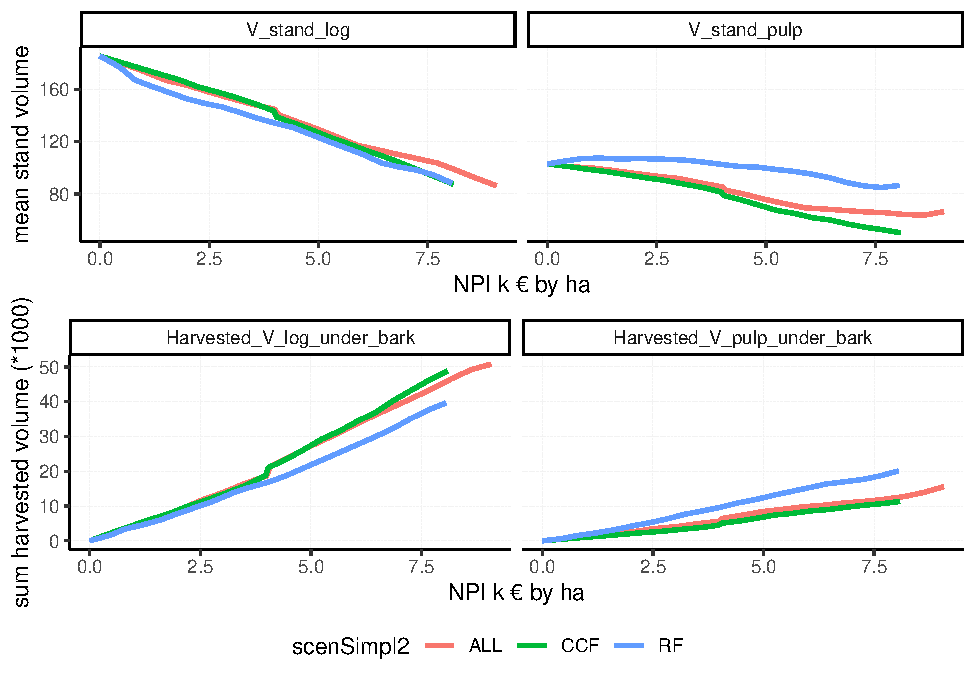
\includegraphics{test_manus_files/figure-latex/plot_V_timber-1.pdf}

\section{Close chunk}\label{close-chunk}

\section{rESULTS}\label{results}

\section*{References}\label{references}
\addcontentsline{toc}{section}{References}

\hypertarget{refs}{}
\hypertarget{ref-Dirac1953888}{}
Dirac, P., 1953. The lorentz transformation and absolute time. Physica
19, 888--896.
doi:\href{https://doi.org/10.1016/S0031-8914(53)80099-6}{10.1016/S0031-8914(53)80099-6}

\hypertarget{ref-Feynman1963118}{}
Feynman, R., Vernon Jr., F., 1963. The theory of a general quantum
system interacting with a linear dissipative system. Annals of Physics
24, 118--173.
doi:\href{https://doi.org/10.1016/0003-4916(63)90068-X}{10.1016/0003-4916(63)90068-X}


\end{document}


